\documentclass[a4paper, 12pt, oneside]{scrbook}
\usepackage[hyphens,spaces,obeyspaces]{url}
\usepackage[sorting = none, backend=bibtex]{biblatex}
\usepackage[german]{babel}
\usepackage[T1]{fontenc}
\usepackage[utf8]{inputenc}
\usepackage[hidelinks]{hyperref}
\usepackage{graphicx}
\usepackage{subcaption}
\usepackage{epstopdf}
\usepackage{lmodern}
\usepackage{float}
\usepackage{acronym}
\usepackage{booktabs}
\usepackage{caption}
\usepackage{csquotes}
\usepackage{enumitem}
\usepackage{fancyhdr}
\usepackage{url}
\usepackage{listings}
\usepackage[table]{xcolor}
\usepackage{wrapfig}
\usepackage{forest}
\usepackage{tabularx}
\usepackage{colortbl}
\usepackage{booktabs}
\usepackage[onehalfspacing]{setspace}
\usepackage{amsmath}
\usepackage{threeparttable}
\usepackage[german]{cleveref}
\usepackage{parskip}

\renewcommand*{\headfont}{\normalfont}
\renewcommand*{\multicitedelim}{\addsemicolon\space}
\renewcommand*{\headrulewidth}{0pt}
\renewcommand*{\arraystretch}{1.5}
\setlength{\parskip}{1.5ex}
\makeatletter
% define new boolean conditional switch for whether
% the abstract is being typeset
\newif\ifabstract
% redefine `\chapter` so it only starts a new page if not typesetting
% the abstract; sets abstract conditional to false after doing so
\renewcommand\chapter{\ifabstract\relax\else%
	\if@openright\cleardoublepage\else\clearpage\fi%
	\fi
	\abstractfalse%
	\thispagestyle{plain}%
	\global\@topnum\z@
	\@afterindentfalse
	\secdef\@chapter\@schapter}

% command for putting the title and name above the abstract; switches
% abstact boolean to true for next `\chapter*` command...
\newcommand{\conclusion}{
	\if@openright\cleardoublepage\else\clearpage\fi
		\begin{center}
			\textbf{\larger{Summary}}\par
			\emph{Hier kommt nach der Fertigstellung der Arbeit noch eine Zusammenfassung der Arbeit mit ein oder mehreren Sätzen hin. Hier kommt nach der Fertigstellung der Arbeit noch eine Zusammenfassung der Arbeit mit ein oder mehreren Sätzen hin. Hier kommt nach der Fertigstellung der Arbeit noch eine Zusammenfassung der Arbeit mit ein oder mehreren Sätzen hin2. }\par
		\end{center}

	\abstracttrue}
\makeatother
\lstset
{
         basicstyle=\footnotesize\ttfamily,
         numbers=left,               	% Ort der Zeilennummern
         numberstyle=\tiny,          	% Stil der Zeilennummern
%         stepnumber=2,               	% Abstand zwischen den Zeilennummern
         numbersep=5pt,              	% Abstand der Nummern zum Text
         tabsize=2,                  	% Groesse von Tabs
         extendedchars=true,
         breaklines=true,            	% Zeilen werden Umgebrochen
         keywordstyle=\color{red},
            frame=b,
 %        keywordstyle=[1]\textbf,    	% Stil der Keywords
 %        keywordstyle=[2]\textbf,
 %        keywordstyle=[3]\textbf,
 %        keywordstyle=[4]\textbf, \sqrt{\sqrt{}}
         stringstyle=\color{white}\ttfamily,
         showspaces=false,
         showtabs=false,
         xleftmargin=27pt,
         framexleftmargin=27pt,
         framexrightmargin=5pt,
         framexbottommargin=4pt,
%         backgroundcolor=\color{lightgray},
         showstringspaces=false      	% Leerzeichen in Strings anzeigen ?
}
\addbibresource{Bachelorarbeit.bib}

\begin{document}
	\frontmatter
	\def\doctype{Bachelorarbeit}
\def\title{Vorgehensweise zur Implementierung der VDMA Spezifikation „OPC UA for Machinery (OPC 40 001)“ in Maschinen und IT-Systemen erarbeiten}
\def\author{Rico Kursidem}
\def\supervisor{Dipl. Ing (FH) Michalowski}
\def\supervisortwo{Prof. Dr. Mielebacher}

\begin{titlepage}

\vspace{10mm}

\begin{center}
	
	\vspace{5mm}
	\huge \title
	
	\vspace{34pt}
	\large \doctype
		
	\vspace{30pt}	
	\small Angewandte Informatik \\
	\large Duale Hochschule Baden-Württemberg Mosbach \\
	\small Studienpartner \\
	\large AZO GmbH \& Co. KG \\
    \vspace{35pt}
    
    
\includegraphics[height=2.5cm]{prefix/image/logo-dhbw.eps}
    
\includegraphics[height=2.5cm]{prefix/image/logo-azo.png}
	
	\vspace{40pt}	
	\small von \\
	\large \author \\
	\small betreut von \\
	\large \supervisor \\
	\small und \\
	\large \supervisortwo

\end{center}

\vspace{75pt}


\vspace{49.7pt}

\fancypagestyle{empty}{
  \fancyhf{}
  \fancyfoot[C]{\today}
}

\end{titlepage}
	\chapter*{Abkürzungsverzeichnis} 
\begin{acronym}
	%A
	\acro{API}{Advanced Programming Interface}
	%B
	%C
	\acro{COM}{Component Object Model}
	%D
	\acro{DCOM}{Distrebuted Component Object Model}
	%E
	\acro{ERP}{Enterprse Recource Planning}
	%F
	%G
	%H
	\acro{HMI}{Human Maschine Interface}
	%I
	\acro{IoT}{Internet of Things}
	%J
	%K
	%L
	%M
	\acro{M2M}{Maschine-zu-Maschine}
	\acro{MES}{Manufacturing Execution System}
	\acro{MQTT}{Message Queuing Telemetry Transport}
	%N
	%O
	\acro{OPC UA}{Open Platform Communications Unified Architecture}
	%P
	%Q
	%R
	%S
	\acro{SOA}{Service orientierte Architektur}
	%T
	\acro{TCP/IP}{Transmission Control Protocol/Internet Protocol}
	%U
	\acro{UMATI}{Universal machien technology interface}
	%V
	\acro{VDMA}{Verband Deutscher Maschinen- und Anlagenbau}
	\acro{VDW}{Verein Deutscher Werkzeugmaschinenfabriken e.V. }
	%W
	%X
	%Y
	%Z
\end{acronym}
	\tableofcontents
	\listoffigures
	\listoftables
	%\lstlistoflistings
	\nocite{*}

	
	
	\chapter*{Abstract}
	
	\section*{Deutsch}
	
	\section*{English}
	
	
	\mainmatter
	\pagebreak
%	\conclusionpng
	\chapter{Einführung}\label{ch:Einführung}
	% (4 Seiten)
	
	Die moderne Welt wird zunehmend vernetzter. Unternehmen weiten ihre Wertschöpfungsketten global aus und erzeugen so ein weltweites Abhängigkeitsnetz. Unternehmen erweitern Ihren Kundenmarkt auf die gesamte Welt und beziehen von überall Zulieferungen. In der Industrie ist es dabei besonders wichtig, dass alle Teilnehmer an Wertschöpfungsketten, Arbeitsgruppen und Verträgen dasselbe Verständnis von Daten haben. Um ein weltweit, einheitliches und unmissverständliches Kommunikationssystem zu ermöglichen, werden Standards verwendet. In Zeiten der Industrie 4.0 nehmen Standardisierungen einen noch wichtigeren Platz ein als zuvor. Da Anlagen immer mehr aus Maschinen verschiedenster Hersteller zusammengesetzt sind, ist ein gemeinsamer übergreifender Kommunikationsstandard besonders wichtig, um eine fehlerfreie, effiziente und wirtschaftliche Produktion zu ermöglichen.
	
	Standardisierung wird verwendet, um effizienteren Austausch und effektivere Prozesse durchzuführen. Ein sehr altes Beispiel sind Sprachen. Eine Menge an Regeln, welche zur Kommunikation genutzt werden, auf die sich alle Teilnehmenden geeinigt haben. In dieser Arbeit soll es um die Standardisierung im Bereich der \ac{M2M} Kommunikation gehen. Durch die Herausforderungen von Industrie 4.0 kann ein guter Standard die Integration mehrerer Systeme vereinfachen und Kosten sparen.
	
	In der M2M Kommunikation existieren bereits Standards, die schon vor Industrie 4.0 entworfen wurden. Dazu gehört auch \ac{OPC UA}. \ac{UMATI} baut auf diesem Standard auf und verspricht weitere Aspekte wie beispielsweise eine Umgebung in der neue Maschinen durch Plug \& Play integriert werden können. Das Ziel von \ac{UMATI} ist es, die zahlreichen Implementationen von OPC UA Schnittstellen zu standardisieren und zusammenzufassen, um so für Produzenten von Anlagen und Software einen gemeinsamen Standard zu finden. Das Ziel dieser Arbeit ist \ac{UMATI} zu analysieren, die Implementation dieses Standards zu erforschen und ein Proof-of-Concept zu entwickeln, der die Fähigkeiten dieser Schnittstelle demonstriert.
	
	\section{Problemstellung und Ziel}
	
	% (1-2 Seiten)
	
	 Durch die zunehmende Automatisierung der Produktion und Fertigung stehen viele Produzenten vor der Aufgabe, zahlreiche Maschinen verschiedenster Hersteller in ihren Fertigungsprozess zu integrieren. Viele dieser Maschinen nutzen verschiedene Kommunikationsprotokolle, Datenformate und Schnittstellen, was die Integration dieser diversen Systeme erschwert. Durch eine komplizierte Integration kann Vendor Lock-in entstehen. Dieses Konzept beschreibt die Bindung eines Kunden an einen Anbieter, da dieser eine Technologie oder Kommunikationsstrategie integriert, die andere Hersteller nicht oder nur extrem schwer integrieren können. Dies kann zu einer Atmosphäre führen, welche für den Kunden weniger Flexibilität und Kontrolle über seine eigene Produktion gibt und gleichzeitig die Kosten steigen lässt. Um dieses Problem zu lösen, müssen sich die Produzenten zu einem Standard zusammenfinden und die Interoperabilität ihrer Systeme zu gewährleisten. \cite{mielebacher_verteilte_2021}
	 
	 Für AZO als Anlagenproduzent ist es von großem Interesse, mit Anlagen und Maschinen anderer Hersteller kommunizieren zu können und dabei die Integration möglich einfach zu realisieren. Auch für Entwickler von \ac(MES) bedeutet die Standardisierung von Kommunikationsprotokollen eine schnellere und einfachere Entwicklung, was zu niedrigeren Entwicklungskosten führt und die Robustheit der Systeme erhöht. AZO nimmt an der Entwicklung von \ac{UMATI} teil, um diese Standardisierung zu erreichen. Dieser Standard möchte die Schnittstellen für die Kommunikation zwischen Maschinen und auch mit der darüber liegenden Datenverarbeitung definieren und basiert auf dem offenen Standard \ac{OPC UA}.
	 
	 Das Ziel dieser Arbeit ist es, \ac{UMATI} in einem Testumfeld anhand eines Proof-of-Conzept aufzubauen. Um dies zu erreichen, soll zunächst eine Marktanalyse durchgeführt werden und mögliche Lösungen zum Versenden und Empfangen von Daten zwischen Maschine und \ac(MES) zu finden. Diese sollen anhand von selbst entwickelten Kriterien abgewogen und bewertet werden. Die vielversprechendsten Umsetzungen sollen in einem Testsystem implementiert werden und für zukünftige Demonstrationen auf Messen für AZO zur Verfügung gestellt werden. Außerdem soll evaluiert werden, ob \ac{UMATI} auch in der Low-Code Plattform Node Red angewendet werden kann und wenn möglich, das entstehende System als Open-Source Lösung der Öffentlichkeit zur Verfügung zu stellen.
	 
	 Der Prototyp soll ebenfalls eine Integration in ACAS umfassen. Damit kann gezeigt werden, dass die Schnittstellen von AZO Anlagen mit \ac{UMATI} realisierbar sind. Diese Integration muss im Nachgang weiter evaluiert werden, um festzustellen, ob UMATI als Standardisierung eine geeignete Lösung ist.
	
	%TODO Relevanz für AZO und Wissenschaft
	%TODO Sicherheitsrelevanz
	
	\section{Unternehmen}
	
	 Diese Arbeit wird mit dem Dualen Partner \textit{AZO Gmbh \& Co. KG} durchgeführt. AZO bietet maßgeschneiderte Lösungen für die automatisierte Förderung, Lagerung und Dosierung von Rohstoffen weltweit an. Dabei werden Anlagen für die Bereiche der Chemie-, Nahrungsmittel-, Pharma-, Kosmetik und Kunststoffindustrie gefertigt. Diese Projekte umfassen die Planung, Fertigung und Montage, sowie die Automatisierung der Anlagen.
	 
	 AZO entwickelt ein eigenes MES-System ACAS, welches die Kommunikation zwischen Anlagen von AZO, aber auch Anlagen von anderen Herstellern, mit den Kunden vereinheitlichen und verbessern soll. Dabei soll ein umfassendes System entstehen, welches Steuerung, Visualisierung und Überwachung der Produktion übernehmen und in einer zentralen Software bündeln soll.
	 
	 ACAS entsteht in der Entwicklungsabteilung, welche ebenfalls an dieser Arbeit beteiligt ist. Sie fokussiert sich auf die Automatisierung von AZO Anlagen im Bereich von SPS, Steuerungen bis zur Datenverarbeitung und Erhebung auf abstrahierter Ebene. 
	
	%TODO: Was stellt mir AZO zur verfügung - System, Server, ...
	
	\section{Forschungsfragen}
	
	Die Standardisierung der Integration von verschiedensten Maschinen in eine Umgebung ist nötig und kann zu verstärkten Effizienzsteigerungen und Aufwandsersparnis führen. Für Anlagenbauer verspricht die Nutzung von Umati, diese Integration in einen schnellen und effizienten Prozess zu wandeln. Um das Potenzial von Umati zu evaluieren, wurden folgende Schwerpunkte betrachtet:
	
	\begin{itemize}
		\item \textbf{Q1}: Welche Herausforderungen ergeben sich bei der Umsetzung von Umati?
		\item \textbf{Q2}: Welche Lösungen zur Umsetzung von Umati sind am Wirtschaftlichsten?
		\item \textbf{Q3}: Wie kann die Datenkommunikation von Anlage und ACAS bestmöglich implementiert werden?
	\end{itemize}
	
	\section{Aufbau der Arbeit}
	
	Nachfolgend werden Thematiken beschrieben die zum grundlegenden Verständnis der Arbeit beitragen (Kapitel \ref{ch:Grundlagen}). Daraufhin werden die Methodiken beschrieben, mit denen die Informationen für diese Arbeit erhoben wurden (Kapitel \ref{ch:Methodiken}). Im Hauptteil der Arbeit (Kapitel \ref{ch:Ergebnisse}) wird der restliche Ablauf der Arbeit beschrieben. Es werden zunächst Informationen zur Entscheidungsfindung eingeholt und in Analysen in Relation gesetzt und daraufhin wird die Entwicklung des Prototyps beschrieben. Die Arbeit schließt mit einer Diskussion der gefundenen Ergebnisse und einem Fazit (Kapitel \ref{ch:Diskussion_Fazit}).
	
	% TODO: Messematerial wenn in kapitel behandelt noch anhängen
	
\chapter{Grundlagen}\label{ch:Grundlagen}
	% (16 Seiten)
	
	% Stand der Technik
	
	
	\section{OPC UA}
	
	 \ac{OPC UA} ist ein unternehmensunabhängiger, offener Standard zur Kommunikation von Informationen und Daten zwischen Maschinen im industriellen Umfeld. Das Protokoll wurde 2008 von der OPC Foundation veröffentlicht und nimmt sich zur Aufgabe, die Interoperabilität von Systemen zu fördern. Es verwendet eine \ac{SOA} und kann auf verschiedensten Betriebssystemen verwendet werden. OPC UA ist sehr gut skalierbar und kann deshalb als Kommunikationsprotokoll bei kleinen \ac{IoT} Systemen als auch bei komplexen Cloud-Systemen zur Anwendung kommen. 
	 
	 OPC UA baut auf einem Server-Client-Modell auf, wobei der Client die Anfragen an den Server senden muss. Der Client fragt den Server nach Daten und analysiert diese während der Server stellt die Daten zur Verfügung. Diese Struktur ermöglicht eine einfache Skalierung von verschiedensten Geräten. 
	 
	 Das Ziel von OPC UA und auch im weitergetragenen Sinne von Umati ist das Erreichen von Interoperabilität im industriellen Bereich. Interoperabilität beschreibt die Standardisierung von Kommunikation zwischen Systemen. Allgemein kann diese in 4 Stufen eingeteilt werden, wobei jede Ebene auf die darunterliegende aufbaut. Im Schaubild \ref{fig:Interoperabilität} sind die vier Ebenen Strukturelle, Syntaktische, semantische und Organisatorische Interoperabilität abgebildet.
	 
	 \begin{figure}[H]
	 	\centering
	 	\includegraphics[width=0.9\textwidth]{res/diagramms/Interoperabilität.pdf}
	 	\caption{Die vier Ebenen der Interoperabilität}
	 	\label{fig:Interoperabilität}
	 \end{figure}
	 
	 Die strukturelle Interoperabilität beschreibt Verbindungen zwischen den Systemen, weshalb sie auch oft als Konnektivität bezeichnet wird. Der Datenaustausch kann nur erfolgen, wenn die beteiligten Systeme miteinander verbunden sind und ein geeignetes \ac{API} implementieren. Diese Verbundenheit kann über ein Netzwerk mit TCP/IP oder HTTP erreicht werden oder kann ein Übertragungsmedium wie USB festlegen. \cite{mielebacher_verteilte_2021}
	 
	 Sind Systeme syntaktisch interoperabel, nutzen und verstehen sie die Struktur der Daten. Hierfür können festgelegte Standards wie XML oder Json verwendet werden. \cite{mielebacher_verteilte_2021-1}
	 
	 Die semantische Interoperabilität beschreibt das vereinheitlichte Verständnis der Daten. Kommunizieren zwei Systeme miteinander, so müssen Sie unter denselben Daten auch dasselbe verstehen. Ein Beispiel für einen Standard, der semantische Interoperabilität umsetzt, ist der "International Classification of Diseases". Bei diesem geht es um die Kommunikation von Krankheiten zwischen Ärzten und wurde von der WHO eingeführt. Jede Krankheit hat einen festgelegten Code, wodurch eine eindeutige Kommunikation gewährleistet ist. \cite{mielebacher_verteilte_2021-1}
	 
	 OPC UA legt anhand des Information-Models die Syntax und Semantik der Daten fest, wodurch die syntaktische Interoperabilität gewährleistet ist. Die semantische Interoperabilität wird anhand der Companion Standards erweitert. Diese beschreiben Technologie-spezifische Informationsmodelle. Diese Standards entstanden durch intensive Kooperation und Zusammenarbeit mit Organisationen, um die Standards möglichst umfassend aufzustellen. \cite{mielebacher_verteilte_2021-1}
	 
	 OPC UA entstand aus dem zuvor entwickelten Standard OPC Classics. Der alte Standard setzte die Kommunikation im Bereich der Automatisierung bereits sehr gut um. Der Nachteil an Classics war jedoch die fehlende Plattformunabhängigkeit. OPC UA unterstützt heute jegliche Betriebssysteme für Clients als auch für die Server. Der Vorgänger musste auf einem Windowssystem betreiben werden. Auch die Kommunikation war auf die von Microsoft entwickelte Technologien \ac{COM} und \ac{DCOM} basiert. Durch die Ablösung dieses Standards durch OPC UA wird über TCP/IP und SOAP kommuniziert, welche beide Plattformunabhängig sind und somit kann zunehmend OPC UA auch auf anderen Plattformen wie Linux, Mac und Android angewandt werden. \cite{mielebacher_verteilte_2021-1}
	
		\subsection{Struktur}
		
		OPC UA ist eine Sammlung von Standards, welche in unterschiedlichen Spezifikationen definiert sind. Diese gliedern sich in eine hierarchische Struktur, welche dann bei der Implementierung aufeinander aufbauen. In Abbildung \ref{fig:OPCUA_Framework} ist die Struktur des UA Framework abgebildet. Im unteren Teil und somit der Grundbaustein dies Modells stehen Spezifikationen zum Transport und der Service Discovery. Diese beschreiben über welche Medien Daten transportiert wird und wie erkannt werden kann, welche Services angeboten existieren, die den OPC UA Standard implementieren. \cite{mahnke_opc_2009, rinke_was_2022}
		
		Zur Infrastruktur, welche im Allgemeinen die Konnektivität gewährleistet, ist auch die Spezifikation für den Datenzugang (Information Access) definiert. Außerdem werden auch weitere Standards beschrieben, um die Sicherheit und Robustheit des Systems zu gewährleisten.
		
		Auf den Standards der Infrastruktur bauen die Spezifikationen der Informationsmodelle auf. Diese bestehen aus den offiziellen OPC UA Spezifikationen und den darauf aufbauenden Companion und Vendor Informationsmodellen. \cite{mahnke_opc_2009}
		
		Die offiziellen Standards befassen sich mit dem allgemeinen Austausch von Daten. Hierzu gehören der Austausch von Echtzeitdaten (DA), historischen Daten (HA) und Alarmen (AC). Neben diesen Hauptfaktoren werden auch andere Standards festgelegt, die das offizielle OPC UA Information Modell bilden. \cite{mahnke_opc_2009, rinke_was_2022}
		
		Auf dem OPC UA Standard setzen die Industriestandardinformation Modelle auf. Diese sind von mehreren Teilhabern entwickelte Standards, die beispielsweise innerhalb einer bestimmten Branche oder Industrie-Gruppen verwendet werden. Diese Standards stehen in den Companion Spezifikationen. Beispielsweise gibt es einzelnen Spezifikationen für AutoID Systeme oder Spritzgussmaschinen, die Abwandlungen und Spezialisierungen haben, die auf ihren Bereich angepasst sind. \cite{mahnke_opc_2009, rinke_was_2022}
		
		Auf der obersten Ebene des Schaubilds in Abbildung \ref{fig:OPCUA_Framework} sind die Vendor Informationsmodelle dargestellt. Diese sind weitere Standards, die die Companion Standards erweitern und innerhalb einer Maschinenumgebung eines Erstellers umgesetzt werden. In diesen Standards sind Veränderungen individueller Hersteller definiert, damit eine weitere Spezialisierung über die Companion Spezifikationen hinaus stattfinden kann. \cite{mahnke_opc_2009, rinke_was_2022}
		
		
		\begin{figure}[H]
			\centering
			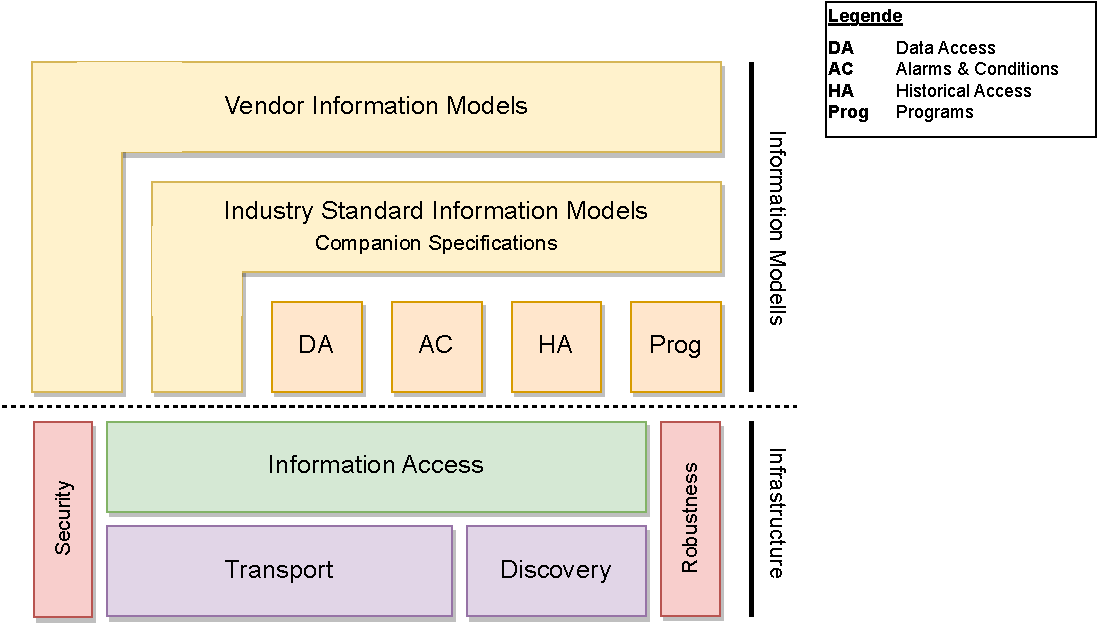
\includegraphics[width=0.9\textwidth]{res/diagramms/companionSpezifikations.pdf}
			\caption{Aufbau des OPC UA Standards, \\ Angelehnt an: Abbildung 1.7 in \cite{mahnke_opc_2009}} %TODO anständig machen
			\label{fig:OPCUA_Framework}
		\end{figure}
	
		\subsection{Kommunikationsaufbau} 
		
		OPC UA besteht aus drei Komponenten, deren Zusammenwirkung in Abbildung \ref{fig:OPCUA_Structure} abgebildet ist. Mehrere Field Connections, die die Sensorik oder SPS darstellen, mit welchen kommuniziert werden soll. Die Daten sollen zu den OPC UA Clients geleitet werden. Dies können \ac{HMI} oder MES-Systeme sein, die die Daten der Maschinen auswerten oder Steuerungsbefehle absenden möchten. OPC UA standardisiert diese Kommunikation über den OPC UA Server. Dieser setzt den OPC UA Standard um und stellt die notwendigen APIs zur Verfügung. \cite{rinke_was_2022}
		
		Der OPC UA Server implementiert die proprietären Kommunikationsprotokolle, die vom Maschinenhersteller entwickelt wurden, um mit den Anlagen und den Field Conections zu kommunizieren. Je nach Art der Daten, die die Maschine weiter gibt, werden die Daten auf dem OPC UA Server abgespeichert oder an den Client weiter gegeben. Ein OPC UA Server kann in zwei Formen entstehen. Der Hersteller kann seiner Maschine die OPC UA Standards bereits bei der Entwicklung einprogrammieren. Damit ist der Server in der Maschine integriert und die Maschine ist so von Beginn an OPC UA fähig. Sollte der Hersteller die Spezifikationen jedoch nicht implementieren, kann der Server auch zusätzlich zwischen die Maschine und den Client geschallten werden. Durch die Unabhängigkeit des Herstellers sind diese Server oft mit mehr Kommunikationsprotokollen ausgestattet, was deren Möglichkeiten, mit der Maschine zu interagieren erhöht. \cite{rinke_was_2022}
		
		Die Kommunikation mit dem Client läuft dabei 1 zu 1 ab. Allerdings kann auch ein 1 zu n Kommunikationsmodell über Publish and Subscribe implementiert werden. Um diese Funktion jedoch zu nutzen, muss der Server mit der OPC UA Pub/Sub Spezifikation erweitert werden. \cite{mielebacher_verteilte_2021}
		
		Der Client kann die Daten über die standardisierte API des OPC UA Servers abfragen. Es können Echtzeitdaten, historische Daten abgerufen werden. Außerdem gibt es eine Spezifikation, wie Alarmierungslogik umgesetzt werden soll. Dies wird anhand der Implementation auf Serverebene deutlich vereinfacht, da sie dann Hersteller unabhängig ist. \cite{rinke_was_2022}
		
		\begin{figure}[H]
			\centering
			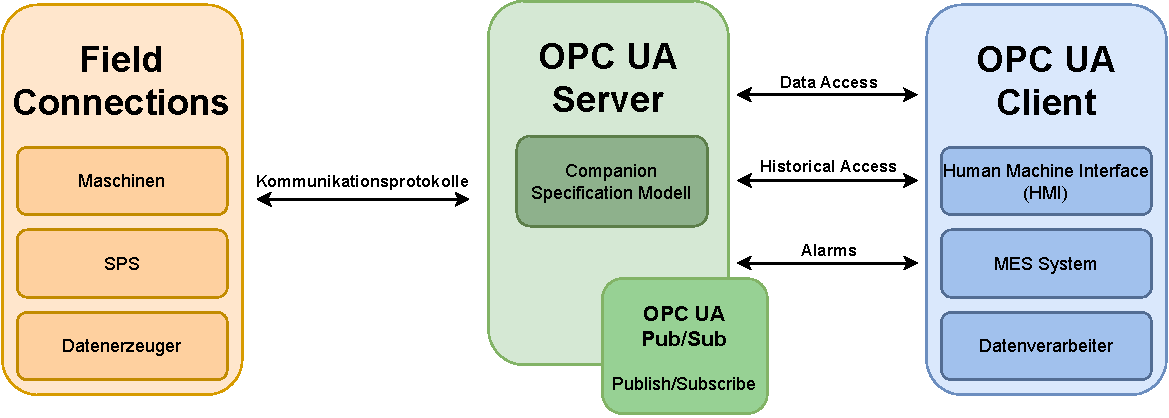
\includegraphics[width=0.9\textwidth]{res/diagramms/OPCUA.pdf}
			\caption{Kommunikationsstruktur OPC UA}
			\label{fig:OPCUA_Structure}
		\end{figure}
	
		% TODO Kommunikationsprotokolle Analyse Anteile, verwendung
		
		
		
		\begin{figure}[H]
			\centering
			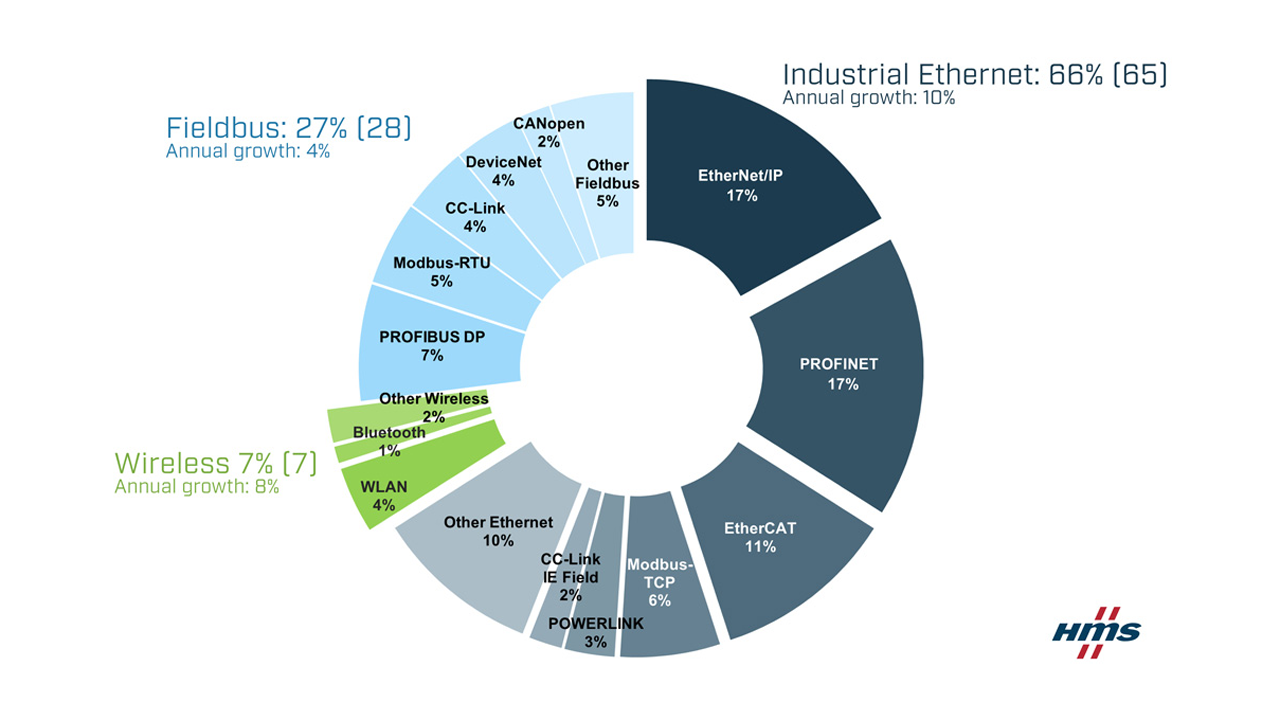
\includegraphics[width=0.9\textwidth]{res/network-shares.png}
			\caption{2022 Industrial network market shares according to HMS Networks \cite{noauthor_2022_nodate}} 
			\label{fig:share}
		\end{figure}
		
		\subsection{Sicherheit}
		
		% (0,5 bis 1 Seite)
		
		Eines der Ziele von OPC UA ist es, eine sichere Verbindung und Kommunikation zu ermöglichen. Deshalb trägt bereits die zweite Spezifikation von OPC UA den Namen 
		\glqq Security Modell\grqq. Hierin ist festgelegt, welche Sicherheitsmechanismen bei der Nutzung von OPC UA angewendet werden sollen.
		
		Die OPC Foundation beschreibt Unified Architecture sicher und Firewall freundlich. OPC UA unterstützt Security auf Transport- und Applikationsebene anhand von selbst entworfenen Protokollen und Erweiterungen von bereits bestehenden Standards. Die Codierung findet auf binärer Ebene statt, wobei die Kommunikation über HTTPS abläuft. Die Authentifizierung von Clients und Servern findet über X509 Zertifikate statt, wobei der Entwickler der UA Anwendung die Anbindung an einen Zertifikatsspeicher selbst übernehmen kann. \cite{noauthor_unified_nodate, noauthor_opc_nodate}
		
		Auf Applikationsebene gibt es Sicherheitsmechanismen, welche dir Authentifikation und Autorisierung der Nutzer bearbeiten. Hierbei kommen Passwörtern, Zertifikaten, Webtokens und weiteres zum Einsatz. Außerdem können mit Rechten für Nutzer weitere Einschränkungen auf den Zugriff einzelner Nutzer gelegt werden. Zuzüglich können Aktivitäten von Nutzern und dem System geloggt werden, um die Nachvollziebarkeit zu erhöhen und die Sicherheit des Systems zu stärken. \cite{noauthor_unified_nodate, noauthor_opc_nodate}
		
		Das Bundesamt für Sicherheit in der Informationstechnik führte 2017 eine Sicherheitsanalyse in Kooperation mit TÜV Süd aus und konnte kleine systematischen Fehler in der Sicherheit entdecken. Sie schreiben OPC UA eine hohe Sicherheit zu, wenn die  Mode Sign und security Mode SignAndEncrypt verwendet werden. \cite{damm_opc_2017}
		
		
		% Wenn bei Umati sich etwas ändert, dann dort noch ein Kapitel puschen
	
	\section{Umati}
		
		%Einführung
		Umati ist eine globale Initiative zur Standardisierung von Interfaces zur Kommunikation zwischen Produktionsanlagen. Sie wird vom \ac{VDMA} und dem \ac{VDW} verwaltet und vorangetrieben von den zahlreichen Mitgliedern der beiden Vereinigungen. Das Ziel ist es, die Kommunikation zwischen Maschinen möglichst einfach, sicher und einfach zu gestalten. Es soll eine Plug \& Play Umgebung entstehen, in der neue Maschinen in eine Anlage durch bloßes Einstecken ins Kommunikationsnetzwerk integriert werden können. Die Umati Initiative entwickelt Standards, welche weltweit zum Einsatz kommen sollen, um eine starke internationale Gemeinschaft um diesen Standard zu erreichen. \cite{noauthor_umati_2023}
		
		%OPC UA in UMATI
		\ac{UMATI} baut auf den OPC UA Standards der OPC Foundation auf. OPC UA bildet dabei die Basis und definiert, wie und was kommuniziert werden soll. Es legt fest, was die Rahmenbedingungen für Konnektivität und syntaktische Interoperabilität sind. \cite{noauthor_umati_2023} OPC UA ermöglicht es die Semantische Interoperabilität über Companion Spezifications zu versichern. Diese werden auch schon in der Industrie eingesetzt weshalb sich \ac{UMATI} die Aufgabe gemacht hat, die verschiedenen Spezifikationen zu vereinheitlichen damit beispielsweise die Identifizierung einer Maschine immer gleich abläuft.
		
		% Automatisierungspyramide
		Umati soll vor allem die vertikale und horizontale Integration im Unternehmen erleichtern. In Abbildung \ref{fig:Automatisierungspyramide} ist die Automatisierungspyramide nach Siepmann abgebildet. Je tiefer die Ebene in der Pyramide liegt, desto vielfältiger sind die Systeme dieser Ebene. Während ein Unternehmen nur ein \ac{ERP} System verwendet, kann es zahlreiche SPS und noch mehr Ein- und Ausgabesensoren geben. Diese müssen vertikal integriert werden. Dafür werden Daten von den unteren Ebenen in die Systeme weiter oben zur Verarbeitung überreicht. Bei der horizontalen Integration kommunizieren gleichartige Systeme miteinander. Beispielsweise wenn mehrere SPS Daten austauschen oder Daten Abteilungsübergreifend übergeben werden, wie bei einem Datenfluss von SCM zu CRM System sein. 
		
		\begin{figure}[H]
			\centering
			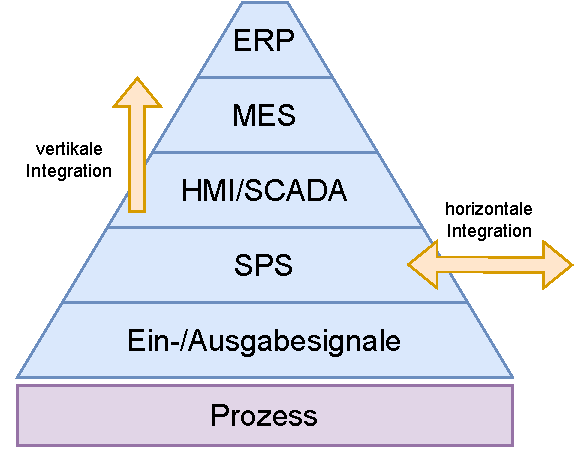
\includegraphics[width=0.8\textwidth]{res/diagramms/Automatisierungspyramide.pdf}
			\caption{Automatisierungspyramide nach Siepmann, \\ Angelehnt an: Folie 8 in \cite{mielebacher_verteilte_2021}} 
			\label{fig:Automatisierungspyramide}
		\end{figure}
		
		Umati legt standardisierte Interfaces fest, mit denen die vertikale und horizontale Integration möglichst einfach umgesetzt wird. Dadurch kann die Wertschöpfung aus Daten kostengünstiger ablaufen und die Analyse, Verarbeitung und Verwertung von Daten, wie es in der Industrie 4.0 üblich ist, besser ablaufen. Umati hat bereits Vorführungen auf Messen veranstaltet, welche die Funktionsfähigkeit einer Umati Umsetzung demonstrieren. Umati standardisiert dabei die Integration von Maschinen, deren Installation und ganze IT Produktionsumgebungen. \cite{noauthor_about_nodate}
		
		%TODO: Umati aufbau
		
		% Companion Specifikations
		Die Semantische Interoperabilität wurde bereits mit OPC UA über die Companion Spezifikationen erreicht. Allerdings entstehen diese Standards in gesonderten Arbeitsgruppen welche auf die Teilnehmer zugeschnitten sind. Dadurch entstehen viele Spezifikationen in vielen verschiedenen Branchen und Maschinen können nicht mehr ohne Übersetzung kommunizieren. Umati versucht diesen Umstand durch das Zusammenfassung dieser Spezifikationen zu beheben. Es sollen Maschinen entstehen, die alle die selbe Sprache sprechen und so einfach in neue IT 
		
		Umati selbst besteht aus verschiedenen Modulen, welche alle Standards für verschiedene Bereiche definieren. In Abbildung \ref{fig:OPCUA_for_machinery} sind alle Interfaces abgebildet, welche auf der Base Spezifikation OPC 40001 aufbauen. Dieser wird auch OPC 40001 UA for Machinery genannt und ist für die Anlagenbauindustrie gedacht. Umati befindet sich noch in der Entwicklung und ist noch nicht vollständig fertiggestellt, deshalb gibt es Interfaces, welche noch nicht umgesetzt, sondern nur geplant sind. \cite{noauthor_machinery_nodate}
		
		\begin{figure}[H]
			\centering
			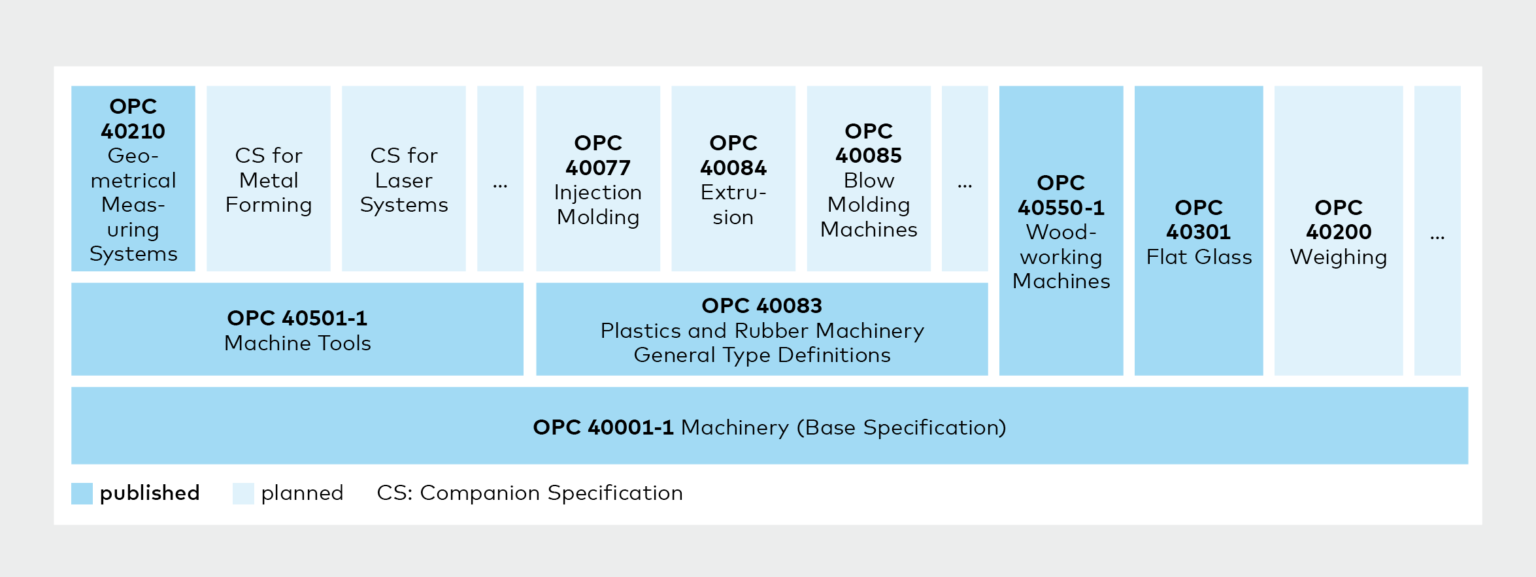
\includegraphics[width=0.9\textwidth]{res/diagramms/OPCUA_for_machinery.png}
			\caption{Interfaces basierend auf OPC UA for Machinery \cite{noauthor_machinery_nodate}} 
			\label{fig:OPCUA_for_machinery}
		\end{figure}
		
		% Kennzahlen, wer nutzt schon, was sind bisherige Meinungen dazu
		
		\subsection{VDMA}
		
		\ac{VDMA} ist der größte Industrieverbund in Europa und hat Umati ins Leben gerufen hat. Der Verband wurde 1892 gegründet und hat seinen Sitz in Frankfurt am Main. Neben der Vertretung der Interessen industrieller Unternehmen in Deutschland und Europa gegenüber der Politik, erarbeitet der VDMA auch Standards und tauscht Know-How zwischen seinen 3.600 Mitgliedsunternehmen aus. \cite{noauthor_verband_nodate} In dem Interessenverband sind Firmen aus den Bereichen Maschinenbau, Anlagenbau und der Zulieferindustrie, welche sich Kompetenzen und Informationen in verschiedensten Themenbereichen von Bildung \& Modernem Arbeiten über Digitalisierung bis zu rechtlichen Feldern teilen. \cite{noauthor_themenubersicht_nodate}
		
		Der VDMA wirkt vor allem mit Förderungen in Bereichen, die Innovation bringen. Beispielweise fördert der Verband Technologien in den Bereichen Industrie 4.0, Digitalisierung und nutzt Lobbyarbeit, um seine Mitglieder auch politisch zu unterstützen. Außerdem veranstaltet der VDMA Messen zur Netzwerkbildung und zum Demonstrieren von neusten Technologien seiner Mitglieder. Im Allgemeinen verfolgt der Verband die Stärkung der europäischen Maschinenbaubranche und die Verbesserung der Wettbewerbsfähigkeit auf internationaler Ebene. \cite{noauthor_themenubersicht_nodate}
		
		AZO, der Partner dieser Arbeit, ist auch ein Mitglied des VDMA. Da AZO ein mittelständisches Unternehmen im Anlagenbau ist, setzt sich der VDMA genau für diese Interessen ein und möchte mit Umati eine Plug \& Play Umgebung im Anlagenbau ermöglichen. Der VDMA möchte eine erhöhte Interoperabilität zwischen den Maschinen ihrer Mitglieder bewirken und so die Wettbewerbsfähigkeit des europäischen Markts stärken, aber auch in der Standardisierung der internationalen Industrie mitwirken. 
		
		\subsection{OPC UA for Machinery}
		
		\texttt{OPC 40001-1/VDMA 40001-1}, auch OPC UA for Machinery, wurde von VDMA und VDM zusammen mit der OPC Foundation entwickelt. Es ist die Base Spezifikation, auf der andere in diesem Bereich aufbauen sollen. Sie wurde im September 2020 veröffentlicht und seit dem aktualisiert worden. Der Standard wird auch in Zukunft erweitert werden, um mehr Use Cases abzudecken.
		
		Im Allgemeinen deckt dieser Standard fundamentale Bereiche ab. Es wird definiert, welche Datentypen genutzt werden können, wie deren Syntax ist und wie sie in Attributen abgespeichert werden können. Es werden Objekte und Klassen festgelegt, wie diese erstellt und definiert werden sollen. Darüber hinaus beschreibt die Spezifikation auch, wie ein Client im System die Maschinen an den OPC UA Servern finden kann. 

\chapter{Methodik}\label{ch:Methodiken}
	% (8 Seiten)
	
	% Forschungsmethodik - Deduktiv??? - Konstruktiv???
	
	\section{Literaturrecherche}
	
	Die Informationen der vorangegangenen Kapitel \ref{ch:Einführung} und \ref{ch:Grundlagen} wurden aus offizieller Literatur entnommen. Zu den Informationen zu OPC UA wurden die offiziellen Spezifikationen und empfohlene Literatur der OPC Foundation verwendet. Dasselbe Vorgehen wurde für die theoretische Vorarbeit von Umati genutzt. Die meisten Informationen zum neuen Standard wurden der offiziellen Webseite des VDMA entnommen. Außerdem sind dort auch Literaturempfehlungen ausgeschrieben welche ebenfalls verwendet wurden. Um theoretische Grundlagen und Konzepterklärungen zu recherchieren, wurden Vorlesungsmaterialien der DHBW Mosbach verwendet.
	
	
	
	% Datenerhebung - Literaturrecherche
	% Stichwort recherche
	
	% Über die Hersteller empfolene Literatur
	
	\section{Evaluation}
	
	% Evaluation des Ergebnisses
	
	Das Ergebnis dieser Arbeit wird ein Prototyp zur Demonstration der Umati Spezifikation sein. Dieser Prototyp muss anhand bestimmter Kriterien bewertet werden. Diese können aus dem Standard ISO 25010 für Softwarequalität entnommen werden. In Abbildung \ref{fig:ISO25010} sind die Softwarequalitätskriterien strukturiert abgebildet, wie sie im ISO-Standard definiert sind. 
	
	\begin{figure}[H]
		\centering
		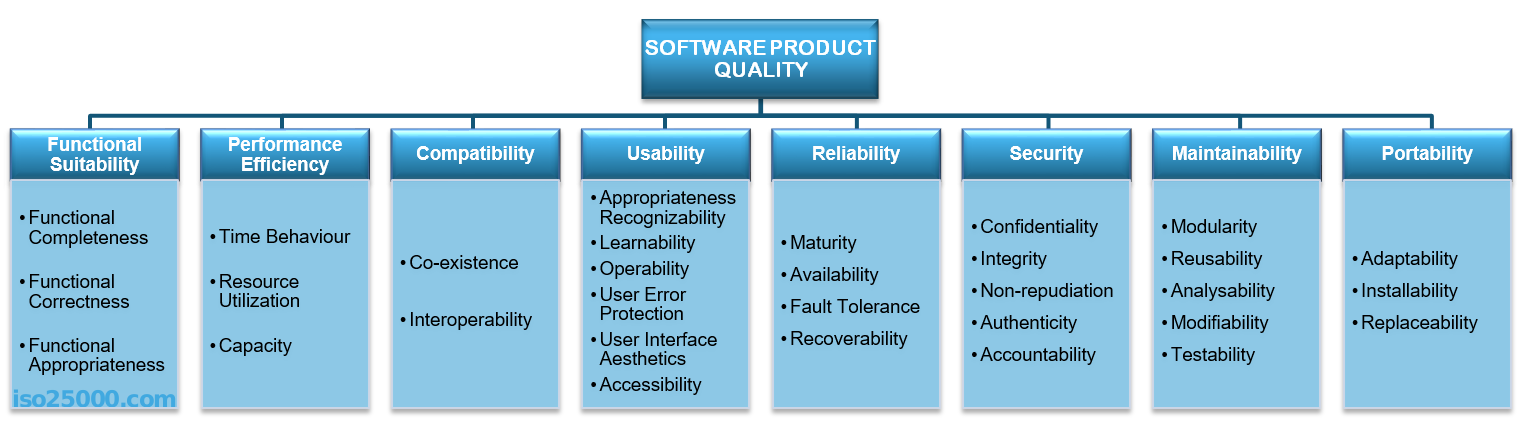
\includegraphics[width=0.9\textwidth]{res/diagramms/iso25010.png}
		\caption{Softwarebewertungskriterien ISO 25010} 
		\label{fig:ISO25010}
	\end{figure}
	
	Die Punkte \textit{Functional Suitability}, \textit{Performance Efficiency}, \textit{Usability} und \textit{Reliability} sind die Hauptkriterien die für den Messeprototypen besonders wichtig sind. Die anderen Kriterien sind ebenfalls von wichtigkeit, können jedoch den anderen nachgestellt werden, da der Prototyp nur demonstrativen Nutzen hat. 
	
	% TODO: Quantifizierbare Ziele setzen
	
	Das Demomaterial welches für die Messe ausgelegt werden soll, muss visuell anschaulich sein und die Kernfunktionen von Umati präsentieren. Es geht darum das Interesse der Messebesucher zu wecken und genug Informationen für ein allgemeines Bild über die Funktionen und Ziele von Umati zu erreichen. 
	
	% TODO: Quantifizierbare Ziele setzen
	
	%TODO: Reflexion
	
	%\section{Experteninterview}
	
	%Im Zuge der Ausarbeitung der Anforderungen an Umati und den Prototyp bot sich die Durchführung eines Experteninterviews an. Es wurde ein semistrukturiertes Interview mit den AZO Mitarbeitern %TODO Name 
	%durchgeführt. Ein semistrukturiertes Interview, auch Leitfaden-gestütztes Interview genannt, geht einen Kompromiss zwischen dem Strukturierten und dem Unstrukturierten Interview ein. Anders als im strukturierten Interview werden die Fragen nicht fest definiert und die Reihenfolge muss nicht zwingend eingehalten werden. Dadurch entsteht ein dynamischeres Gespräch mit dem Experten und der Interviewende kann genauer auf die Spezialbereiche des Experten eingehen. Allerdings verliert die semistrukturierte Methode die Vergleichbarkeit zwischen Interviews, da nicht jede Frage unbedingt bei jedem Interviewten gestellt wird. Um sich von einem unstrukturiertes Interview abzuheben wird bei der Vorbereitung ein Leitfaden erstellt, welcher als Hilfsmittel während des Interviews verwendet werden soll. Dieser spannt den Themenbereich und zweigt die Richtung für das Interview auf. Der Interviewende kann dass Interview thematisch steuern, während der Experte frei sprechen kann. \cite{wesel_semi-strukturierte_2010}
	
	%Die Motivation des Interviews war es, Anforderungen für einen Prototypen zu erarbeiten und dabei die wichtigsten Punkte zu erörtern. Zusätzlich soll ein Meinungsbild und das erwartete Potential des Experten in Bezug auf Umati eingeholt werden. 
	
	%Um ein semistrukturiertes Interview ordnungsgemäß durchführen zu können muss ein Leitfaden entwickelt werden. Dieser soll dem Interview einen klaren Ablauf geben, aber nicht jede Frage bereits vorschreiben. Im Paper Semi-strukturierte Interviews im Software-Engineering werden die 4 Phasen des Experteninterviews beschrieben, welche im Leitfaden widergespiegelt werden sollen. \cite{wesel_semi-strukturierte_2010}
	
	%In der Einführung soll der Interviewte vorgestellt werden und seine Funktionen und Aufgaben beleuchtet werden. Zusätzlich sollen noch Begriffserklärungen stattfinden, um einen Austausch auf gemeinsamen Verständnis zu gewährleisten. \cite{wesel_semi-strukturierte_2010}
	
	%Phase zwei ist die Exploration der derzeitigen Situation. Hierbei muss die derzeitige Infrastruktur behandelt werden und auf den Arbeitskontext eingegangen werden. Außerdem soll ein Bild der derzeitigen Bedingungen, Probleme und Einschränkungen gezeichnet werden. Im Fall des Interviews zu Umati werden hier vorallem Fragen zur Maschine-zu-Maschine Kommunikation und den bis jetzt verwendeten OPC UA Spezifikationen bei AZO. \cite{wesel_semi-strukturierte_2010}
	
	%In der dritten Phase wird dann die zukünftige Situation betrachtet. Hierbei sollen Wünsche und Erwartungen zusammengetragen werden, welche bestimmte Lösungen oder Werkzeuge erreichen können. Der Interviewte kann hier auch eigene Ideen einbringen. Hier kann in Bezug auf Umati die Erwartungen zum neuen Standard ausgedrückt werden und mögliche Anforderungen an den Standard zusammengetragen werden. Dies ist der wichtigste Teil des Interviews, da aus den Antworten aus dieser Phase die Anforderungen an den Prototypen herausgearbeitet werden können. \cite{wesel_semi-strukturierte_2010}
	
	%In der letzten Phase, dem Abschluss, wird der Inhalt des Interviews vom Interviewer zusammengefasst. Daraufhin hat der Interviewte die Möglichkeit, die Vollständigkeit durch weitere Kommentare zu sichern und kann Feedback an den Interviewer geben. Das Interview endet mit einem Dank und dem Abschied. \cite{wesel_semi-strukturierte_2010}
	
	%%TODO Einleitung Leitfaden
	
	%\textbf{Phase 1: Einführung}
	%\begin{itemize}
		%\item \textbf{Begriffsklärungen}: Umati
		
		%\item \textbf{Frage 1}: Wie lange arbeiten Sie bereits bei AZO?
		%\item \textbf{Frage 2}: Was sind Ihre Aufgaben?
		%\item \textbf{Frage 3}: Wie lange haben Sie schon mit M2M Kommunikation und OPC UA zu tun?
	%\end{itemize}
	%\textbf{Phase 2: Exploration der derzeitigen Situation}
	%\begin{itemize}
		%TODO: Probleme bei der kommunikation mit einer Maschine 
		%TODO: Spezifischen Daten (Gleichartige daten, viele verschiedene Daten, ...)
		%\item \textbf{Frage 1}: Wie wird OPC UA bei AZO verwendet?
		%\item \textbf{Frage 2}: Welche Protokolle sprechen die OPC UA Server mit den Maschinen?
		%\item \textbf{Frage 3}: Weisen die Companion Spezifikationen Probleme auf? Gibt es Einschränkungen bei der Kommunikation mit OPC UA?
	%\end{itemize}
	%\textbf{Phase 3: Exploration zukünftiger Situationen}
	%\begin{itemize}
		%\item \textbf{Frage 1}: Erkennen Sie ein Verbesserungspotential bei OPC UA? 
		%\item \textbf{Frage 2}: Was sind Ihre Wünsche/Erwartungen an einen Standard wie Umati?
		%\item \textbf{Frage 3}: Was wären Funktionen, welche besonders Relevant wären bei Umati?
	%\end{itemize}
	%\textbf{Phase 4: Abschluss}
	%\begin{itemize}
		%\item \textbf{1}: Zusammenfassung
		%\item \textbf{2}: Ergänzungen \& Feedback
		%\item \textbf{3}: Abschied und Dank
	%\end{itemize}
	
	%TODO: -> Interview Ergebnisse in Anhang! Und Teilweise in Anforderungsanalyse!
	
	\section{Zeitplanung}
	
	Die Bearbeitungszeit dieser Arbeit sind 12 Wochen. Startend am 19.06.2023 bis zum 11.09.2023. In Abbildung \ref{fig:Grantt} ist ein Grantt-Diagramm zur Zeitplanung abgebildet. In den ersten 4 Wochen sollen die Theoretische Grundlagen und die Analysen der Arbeit abgeschlossen sein um die Praxis am 10.07.2023 beginnen kann. Von Woche 5 bis 10 soll die Implementation und Integration des Prototypen stattfinden. Den gesamten Prozess schätze ich auf gemeinsam 5 Wochen wobei eine zusätzliche Woche als Puffer eingeplant wird, sollte es Verzögerungen wie Krankheit oder Bereitstellungsschwierigkeiten geben. Am 21.08.2023 soll die Arbeit abgabebereit sein und für eine Korrekturlesung bereitgestellt werden. Parallel zur Korrekturlesung sollen die Messedokumente und Schulungsunterlagen angefertigt werden. Die letzten eineinhalb Wochen sollen dann genutzt werden, um die Arbeit zu Korrigieren.
	
	\begin{figure}[H]
		\centering
		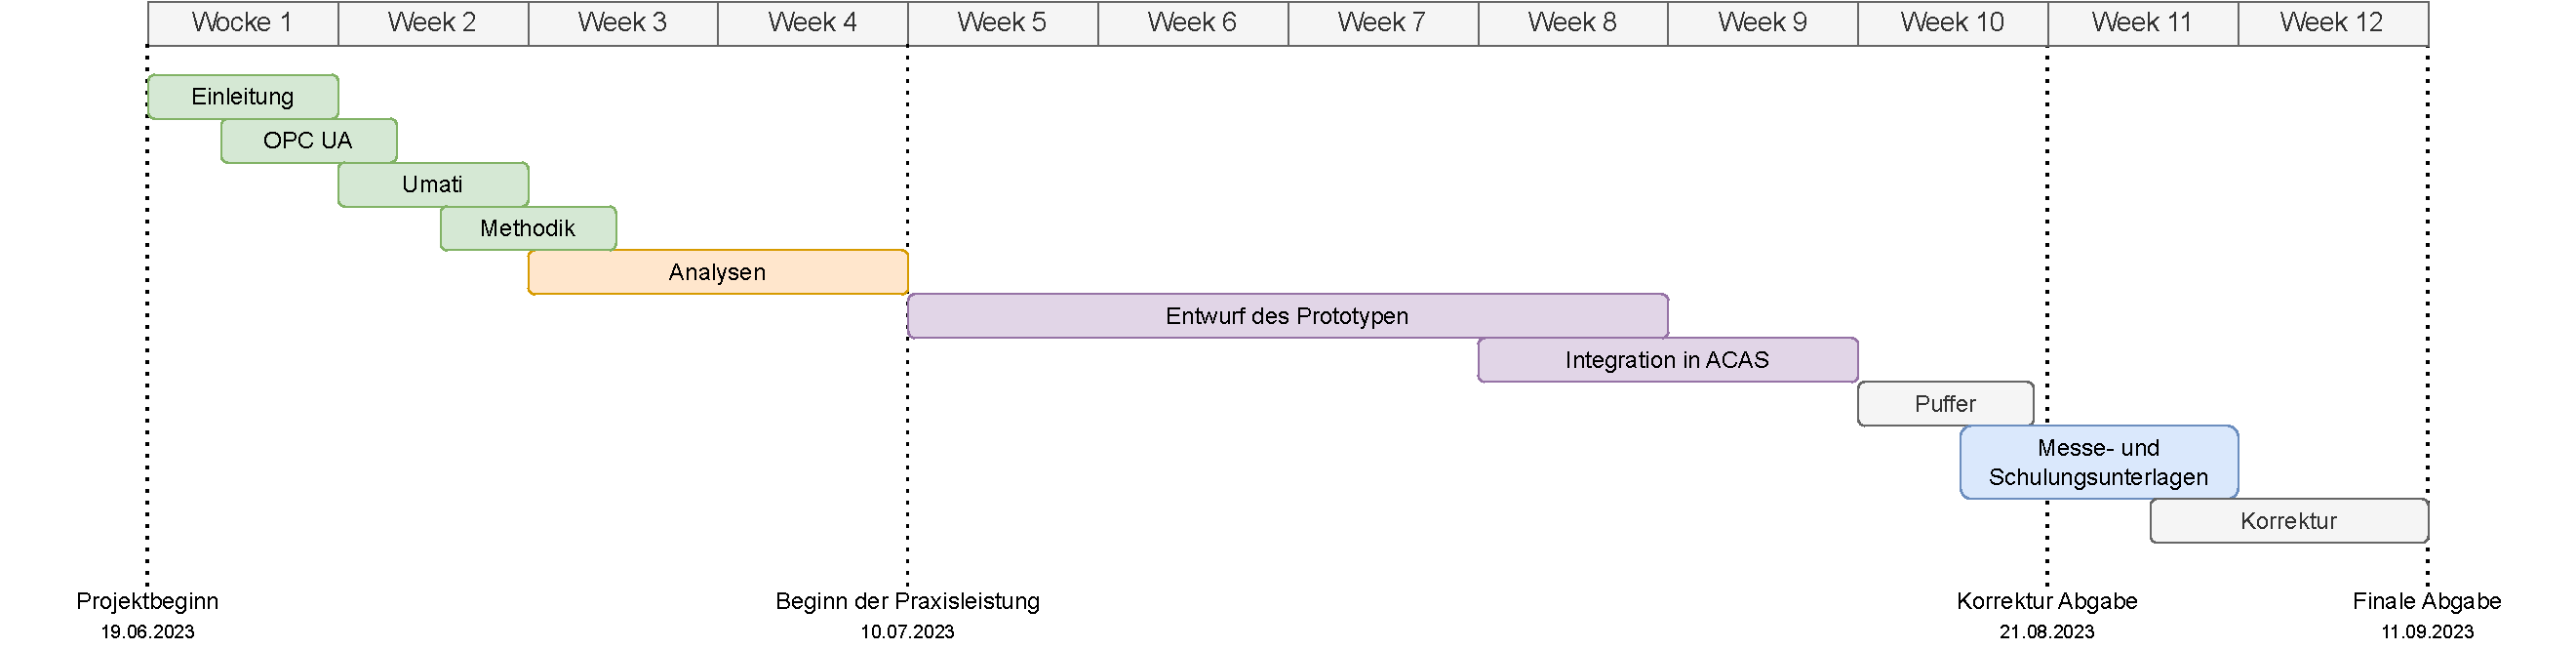
\includegraphics[width=0.9\textwidth]{res/analysen/Grantt-Diagramm.pdf}
		\caption{Grantt-Diagramm zum Projektablauf}
		\label{fig:Grantt}
	\end{figure}
	
	%TODO: Reflexion
	
\chapter{Ergebnisse}\label{ch:Ergebnisse}
	
	% (8 Seiten)
	
	\section{Anforderungsanalyse}
	
		% Experteninterview
		\subsection{Vorgehen}
		
		% Ablaufdiagramm
		
		\subsection{Prototyp}
		Als Grundlage des Umati-Prototypen soll eine Maschine simuliert werden. Es soll keine echte Maschine verwendet werden, da diese eventuell an bestimmten Zeitpunkten ausgeschaltet oder betriebsunfähig sein könnte. Außerdem ist eine Tatsächliche Maschine oder Anlage deutlich kostenintensiver als eine Serverbasierte Simulation. Die simulierte Maschine soll eine Anlage von AZO darstellen, die auch tatsächlich im Einsatz ist. %TODO: welche Maschine machen wir?
		
		Als Beispiel wird ein RoLog simuliert, der bei der automatischen Kleinstmengendosierung von Schüttgütern zum Einsatz kommt. In Abbildung \ref{fig:RoLog} ist ein virtualisierter Aufbau der Anlage abgebildet. Der Roboterarm in der Mitte lagert seine Ressourcenbehälter auf den Schränken an der Seite der Anlage, lagert neue Behälter aus oder ein über die Laufbänder an der Hinterseite (Oben-Links) und dosiert in die Ausgabe an der Front (Vorne-Rechts) des Aufbaus. \cite{noauthor_azo_nodate}
		
		\begin{figure}[H]
			\centering
			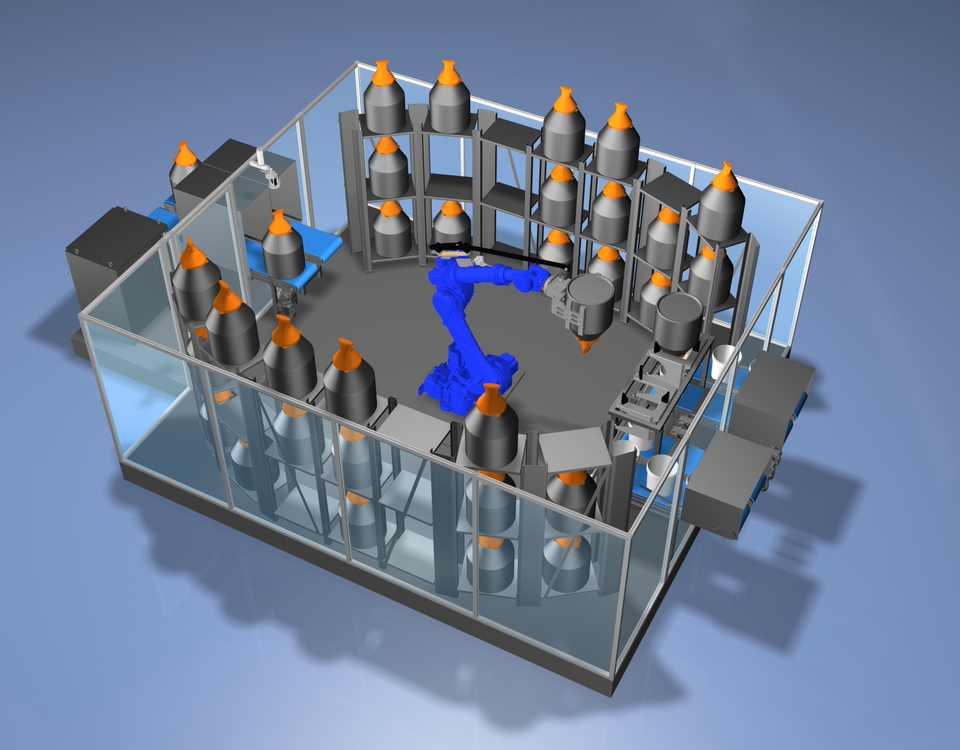
\includegraphics[width=0.7\textwidth]{res/RoLog.png}
			\caption{RoLog von AZO Gmbh \& Co. KG \cite{noauthor_azo_nodate}}
			\label{fig:RoLog}
		\end{figure}
		
		Der Prototyp soll mehrere Funktionen umsetzen. Die Umati Spezifikation soll implementiert werden und soll damit das Senden und Empfangen von Daten ermöglichen. Außerdem soll die Wirkung der Steuerungsnachrichten an die Maschine nachvollziehbar visualisiert werden. In Abbildung \ref{fig:evaluation} sind die Anforderungen an den Prototypen abgebildet. Die Funktionalität beinhaltet dabei das der RoLog mindestens 3 Parameter absenden muss und einen Parameter lesen können muss. Es wird ein Ablauf einer Dosierung eines Rezeptes umgesetzt. Zunächst soll der RoLog durch eine Eingabe gestartet werden. Daraufhin soll er ein Rezept dosieren und einen Alarm ausgeben, wenn er fertig ist. Parallel dazu soll der Zustand der Anlage permanent übertragen werden. %TODO Anforderungen mit Prototyp abstimmen
		
		Bei der Entwicklung des Prototypen soll die Umsetzbarkeit der Schnittstelle über NodeRed geprüft werden. Dies ist von Interesse da NodeRed bei AZO bereits breitgefächert für die M2M Kommunikation angewandt wird. %TODO: Bezug auf ISO 25010
		
		\begin{figure}[H]
			\centering
			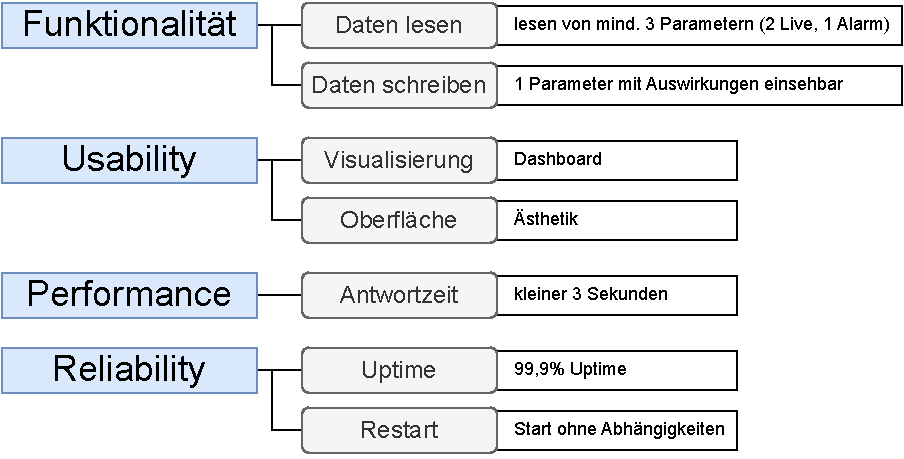
\includegraphics[width=0.9\textwidth]{res/analysen/Evaluation.pdf}
			\caption{wichtigste Bewertungskriterien des Prototypen}
			\label{fig:evaluation}
		\end{figure}
		
	
	\section{Lösungsansätze}
	
		\subsection{Umati Server}
		
		Der VDMA und VDA, die Operatoren von Umati, haben eine Kollektion von Repositories auf Github, auf welchen multiple Implementationsmöglichkeiten eines Umati Servers dargestellt sind. \cite{noauthor_github_nodate} All diese Projekte sind bereits auf Vollständigkeit geprüft und garantieren so die volle umsetzen der Umati-Standards, oder zumindest einer angegebenen Umati Spezifikation. Beispielsweise kann ein Sample-Server verwendet werden, um einen Umatiserver aufzusetzen, der pseudo-zufällige Werte generiert und diese zur Abfrageung bereit stellt. Dieses Repository implementiert zum Zeitpunkt der Abfrage im August 2023 die Spezifikationen \textit{Machine Tool}, \textit{Woodworking}, \textit{Geometrical Measurement Systems} und \textit{Additive Manufacturing} und simuliert Maschinen, welche die notwendigen und optionalen Variablen implementieren, die sie festlegen.
		
		%TODO: Auf interesanteste Repositories eingehen

		\subsection{OPC UA Server - DataFeed}
		
		
		
		
		\subsection{Eigenimplementierung}
		
		Da der Umati Server auf dem Offenen Standard OPC UA aufbaut, kann ein Server auch selbst implementiert werden. Dies hat verschiedene Vor- und Nachteile welche beachtet und auf das Ziel der Implementierung angewandt werden müssen. 
		
		Eigenimplementierungen sind meist Anpassungsfähiger und flexibler, um auf Situationsspezifische Anforderungen zu reagieren. Sie können spezifisch auf den gewünschten Zweck hin optimiert und verbessert werden. Dies kann auch eine einfachere Integration in eine bereits bestehende Umgebung garantieren, da die Anwendung auf diese Umgebung hin angepasst werden kann.
		
		Allerdings kann es auch zu Nachteilen führen. Eigenimplementationen haben, vor allem bei nicht sehr erfahrenen Entwicklern, ein hohes Risiko auf Fehleranfälligkeiten oder Sicherheitslücken. Bei eingekauften Lösungen profitiert die Anwendung im Normalfall von Erfahrungswerten und dem Umstand, dass diese Lösung sich bereits am Markt behaupten musste. Die Fehlende Erfahrung kann auch zu einem Programm führen, welches kaum optimiert und komplex ist, was die Wartbarkeit und Nutzerfreundlichkeit vermindert. Soll die Lösung zu kommerziellen Zwecken eingesetzt werden oder hat hohe Anforderungen an Sicherheit, Zugverlässlichkeit und Robustheit sollte auf eine Eigenimplementation verzichtet werden, da auch der Support für das Produkt wegfällt.
		
		Trotz der Nachteile sollte die Umsetzung einer Eigenimplementierung, vor allem zu Demonstrationszwecken, in Betracht gezogen werden. Hierbei gibt es Low-Code und High-Code Ansätze. Bei High-Code Implementierungen wird die Funktionalität in Code hergestellt. Beispielsweise kann ein OPC UA Server nur anhand von Python implementiert werden. Low-Code Ansätze bedienen sich dabei einem Visuellen Programmierstil. Hierbei wird in besonderen IDEs die Programmierung über Bausteine und möglichst wenig selbst implementierten Code umgesetzt. Beispiele für solche Umgebungen sind NodeRed oder Microsoft Power Apps. 
		
			\subsubsection{High-Code}
			
			Die OPC Foundation stellt ihren Mitgliedern mehrere Implementierungen des OPC UA Servers zur Verfügung. Es kann zwischen C, .NET und Java entschieden werden, wobei alle drei Implementierungen von der OPC Foundation gewartet werden. Die Handhabung der Schnittstellen bleiben größtenteils gleich und damit die Funktionalität der verschiedenen Implementationen der selben Logik folgt, werden alle drei regelmäßig gegeneinander getestet.
			
			%TODO: C
			
			%TODO: .NET 
			
			%TODO: Java
			
			%TODO: UMATI Implementation, Anpassung oder so.
			
			\subsubsection{Low-Code}
			
			
			% Was bracuh ich Hard Soft
			
			% Literaturrecherche an anderen Implementationen (Umati und 5G)
	
	\section{Marktanalyse}
	
		% Fertige Lösungen
		% Node Red selbstimplementierung
	
	\section{Wirtschaftlichkeit und Projektanalyse}
	
		\subsection{Kostenplanung}
		
		\subsection{Fallbeispiel}
			% Beispielswiese an Fallbeispiel -> Durchschnittliche AZO Straße
			% Interview mit Person die diese Integration macht -> Expertenquellen
			% -> Probleme bei Schnittstellen integrierung.
	
	\section{Implementierung eines Prototyps}
	
		\subsection{Aufbau der Umgebung}
		
		\subsection{Implementierung}
		
			% Proof of Konzept
			% Proof of Konzept mit Node Red
			
			% Probleme und Lösungen
		
		\subsection{Integration in bestehende Infrastruktur}
			% Integration in Unternehmensstruktur
			

	
	
	\chapter{Diskussion und Fazit}\label{ch:Diskussion_Fazit}
	
		% (2-5 Seiten)	
	
		% Disskussion -> Subjektive Bewertung der Spezifikation UMATI, ... Literaturpunkte meine Meinung, Sinnvoll Einzusetzen
	
	
	\frontmatter
	\printbibliography

	\chapter*{Interview}
	
	\textbf{text}

\end{document}
